\chapter{Análisis y Diseño}
\label{chap:analisis_diseño}

\lettrine{E}{n} este capítulo se expone brevemente el análisis de requisitos que se ha realizado, así como ya más en profundidad las decisiones tomadas durante el diseño.

\section{Requisitos Hardware}
\label{sec:requisitos_hardware}
En esta sección se analizan los requisitos del proyecto, que han sido divididos en tres secciones en lugar de las tradicionales dos para mayor claridad, ya que el aspecto físico, así como las dimensiones del mismo son un aspecto muy importante a considerar.

\subsection{Requisitos Físicos}
Estos requisitos son de los más importantes debido a que modifican la estructura y limitaciones físicas del proyecto, conteniendo requisitos tanto funcionales como no funcionales, por lo que está en una sección a parte.

Primeramente conviene recordar que este trabajo se lleva a cabo durante la pandemia causada por el COVID-19, por lo que la movilidad es reducida y el teletrabajo desde el domicilio la regla. Bajo estas circunstancias se comienza a realizar un diseño que satisfaga los siguientes requisitos:
\begin{itemize}
    \item El cluster debe ser \textbf{pequeño} y \textbf{manejable}: Debido a que el trabajo se realiza desde casa, éste no puede ser muy extenso, ya que el espacio es muy limitado, por lo que se deben descartar estructuras donde los nodos quedan ``libres'' y ``desperdigados'' encima de una grande mesa.
    \item El cluster debe ser \textbf{visualmente agradable} y \textbf{comprensible}: Debido a que va a ser visto por personas con (posiblemente) escasa formación en \acrshort{hpc}, el cluster ha de tener partes fácilmente identificables, lo más aisladas y señalables posible, y sobre todo no debe abrumar a quien lo ve por primera vez, esto es, no debe sentir que lo que está viendo es ``un montón de cachibaches con cables''.
\end{itemize}

\subsection{Requisitos funcionales}
En cuanto a los requisitos funcionales, como este proyecto se centra más en la divulgación que en la búsqueda de la máxima eficiencia, quizás no se tienen unos requisitos funcionales difíciles de satisfacer, pero \textit{grosso modo} podemos identificar:

\begin{itemize}
    \item En el cluster todos los nodos deben estar conectados entre sí en una topología \textbf{N a N}, es decir, la típica de un switch Ethernet.
    \item El cluster debe ser capaz de ejecutar en general tareas de \textbf{MPI}, y en particular los \acrlong{npb}.
\end{itemize}

\subsection{Requisitos no funcionales}
En cuanto al resto de requisitos no funcionales, principalmente destacar que:
\begin{itemize}
    \item El cluster debe ser \textbf{sensato}: Se debe emplear una calidad y cantidad de materiales adecuada a las expectativas del mismo, esto es que por ejemplo el switch no debería ser el componente más caro de todo el presupuesto, pero tampoco debemos escatimar en él para aprovechar la tarjeta de red Gigabit Ethernet de las Raspberry Pi 4B.
    \item Enlazando con el requisito superior, los componentes a emplear serán actuales y aportarán una relación \textbf{calidad/precio} lo más \textbf{elevada} posible.
    \item El cluster debe ser \textbf{extensible} y \textbf{mantenible}: El despliegue hardware debe permitir modificaciones y mantenimientos de forma moderadamente sencilla.
\end{itemize}

\section{Diseño Hardware}
\label{sec:diseño_hardware}
La etapa de diseño ha consumido una cantidad de tiempo para nada desdeñable, ya que diseñar un sistema que cumpla todos los requisitos no es una labor precisamente trivial. A continuación se exponen los elementos que conforman el ensamblaje del sistema, así como planos que documentan el diseño del mismo.\footnote{El presupuesto, así como otros documentos relativos al presupuestado y compra de materiales se puede encontrar anexado en \#REF\# (TODO RECOLOCAR O COMPLETAR)}

\subsection{Elementos Hardware}
En cuanto a los elementos que conforman el cluster, éste se compone de:
\begin{itemize}
    \item 8x Raspberry Pi
    \item 8x MicroSD 32GB
    \item 1x Switch 8 puertos
    \item 1x Tarjeta de red USB 3.0 a Gigabit Ethernet 
    \item 2x Torres de 4 Raspberry Pi
    \item 1x Ventilador de 120mm
    \item 1x DC-DC Step-Up Variable 
    \item 1x Fuente de alimentación 5V 150W
    \item 8x Cables USB Type-C
    \item 8x Latiguillos Ethernet
\end{itemize}

A continuación se da una explicación detallada de la decisión de estos materiales.

\subsubsection{Raspberry Pi 4B}
Este computador, como se comenta previamente en \nameref{sec:motivacion}, destaca por su reducido formato de forma, del tamaño de una tarjeta de crédito, así como por su bajo consumo y coste. Esto lo hace una solución idónea para este proyecto, que no requiere de hardware muy potente, sino más bien de mucho hardware poco potente que permita simular la estructura de un supercomputador.

%% TODO INSERTAR IMAGEN

\subsubsection{MicroSD}
Una parte que puede pasar desapercibida en una primera aproximación pero que es muy importante son las tarjetas MicroSD, ya que sin ellas las Raspberry Pis no podrán arrancar ningún sistema operativo.\footnote{Desde la versión 2020-09-14 del bootloader se permite el arranque desde dispositivos USB \cite{rpibootloader20200903}}

Se han elegido las tarjetas Samsung Pro Endurance debido a su alta capacidad de escrituras, ya que otros tipos de tarjetas sin este propósito específico podrían sufrir bastante desgaste y llegar al final de su vida útil prematuramente. 

La elección de la versión de 32GB de capacidad, a pesar de que no sean necesarios, es trivial, ya que no existen modelos de menor capacidad y este extra de espacio puede ser bienvenido en hipotéticas futuras iteraciones sobre esta infraestructura.

%% TODO INSERTAR IMAGEN

\subsubsection{Switch Gigabit de 8 puertos}
Una de las partes más interesantes y a las que más vueltas se le ha dado es cómo hacer para conectar los mini computadores sin que se convierta en un lío de cables y sin que el hardware esté desproporcionado. Primeramente destacar que el switch debe funcionar a 5V para poder ser alimentado directamente por la fuente de alimentación, siendo esto un importante requerimiento.
Por otro lado, tambien se debe tener en cuenta que normalmente los switches se fabrican con puertos múltiplos de dos, y esto puede no parecer un problema: hay 8 dispositivos a conectar, por tanto un switch de 8 puertos parece hacer un buen trabajo.

% TODO INSERTAR ANOTHER IMAGEN

Sin embargo esta tarea no es tan sencilla, ya que el cluster debe poder ser accedido desde el exterior, lo que hace necesario un switch de 9 puertos. Estos switches, si bien existen son escasos e innecesariamente caros, y comprar la siguiente opción, siendo ésta el switch de 16 puertos no es una opción.

¿La solución? Añadimos un adaptador \nameref{sssec:usb30age}.

\subsubsection{USB 3.0 a Gigabit Ethernet}
\label{sssec:usb30age}
Con este adaptador, y puenteando las interfaces Ethernet nativa de una Raspberry y la conectada por USB se puede obtener virtualmente un switch de 9 puertos, cierto es que a expensas de un pequeño coste de CPU para manejar esos paquetes de red, que a la hora de la verdad tendrá un marginal impacto, ya que las comunicaciones intensivas se realizarán dentro del propio cluster.

% TODO INSERTAR ANOTHER IMAGEN Y QUIZÁS UN DIAGRAMA DE SWITCH VIRTUAL DE 9

\subsubsection{Torres de \acrshort{rpi}}
\label{sssec:torresrpi}
Las Raspberry Pis se apilan verticalmente como servidores en un rack para poder ser cableadas, accedidas, y refrigeradas de forma sencilla, a resultar visualmente agradables en esta disposición.

Además estos kits incluyen disipadores para RAM, CPU y controlador de USB, así como refrigeración activa, que no se instalará en este caso.

% TODO INSERTAR IMAGEN DE TORRES Y DISIPADORES

\subsubsection{Ventilador de 120mm}
Como se menciona previamente, las \nameref{sssec:torresrpi} incluyen refrigeración activa, pero se ha optado por no incluirla por el nivel de ruido que hacen, a parte de la poca necesidad de la misma dada la naturaleza del proyecto. Sin embargo para permitir la extensibilidad del proyecto en forma de nuevas iteraciones, se ha añadido un ventilador de 120mm optimizado para presión, que mueve aire de un extremo al otro del cluster, refrigerando los mini computadores con ayuda de los disipadores instalados.

Volviendo a hablar de tensiones, el ventilador elegido funciona a 12V. Sin embargo, alimentarlo a esa tensión haría que funcionase a máxima potencia constantemente. Para evitar esto, los fabricantes de ventiladores utilizan principalmente dos aproximaciones: regulación de voltaje y modulación por ancho de pulsos, o \acrshort{pwm}. En la primera de ellas, esa regulación de voltaje se realiza informada por la línea de tacómetro. Sin embargo en este caso,  dados los requerimientos térmicos de los mini computadores empleados, únicamente se empleará un step-up variable con el que se mantiene el ventilador a una velocidad fija (y lo más baja posible para rebajar el nivel de ruido), ignorando la línea de tacómetro. De esta forma el usuario tiene la posibilidad de elevar la potencia en el improbable escenario de que se necesitase más caudal de aire. (Esto ocurriría principalmente si en otra iteración sobre este trabajo se decide hacer overclock al cluster)

% TODO FOTOS (quizás de la construcción??) tambien incluir fotos del step up
%%%                     %%%
%     INSERTAR IMAGEN     %  Tacómetro y pwm, esquemático de conexión fan
%%%                     %%%

\subsubsection{Fuente de alimentación 5V 150W}
La fuente de alimentación es un componente fundamental del cluster, y es que las Raspberry Pi 4 consumen una cantidad de energía nada baja. Solamente el propio dispositivo funcionando a pleno rendimiento consume alrededor de 7.5W, consumo que se dispara si se enchufan periféricos a sus puertos USB. Por esta razón la Raspberry Pi foundation, en lo que debe ser un movimiento para ahorrar problemas a usuarios menos experimentados, recomienda 3A (a 5V) por Raspberry Pi, es decir 15W por dispositivo.

Dadas estas circunstancias, y para ahorrar posibles problemas presentes y futuros, se ha optado por una fuente de alimentación DC de 5V con una potencia de 150W, que sin duda satisface por más del doble los requerimientos energéticos del cluster actual.

% TODO intertar imagen fuente y esquemático conexiones eléctricas (incluir switch y ventilador)

\subsubsection{Cableado Eléctrico y de Red}
Tras la lista de componentes previamente expuestos, únicamente queda tratar la interconexión de los mismos, un componente que da más problemas de lo que pueda parecer.

En cuanto al cableado Ethernet no hay mucho que clarificar. Los cables de 4 pares trenzados Cat5E se cortan a la longitud necesaria, y se crimpan siguiendo la disposición ANSI/TIA-568B.

El cableado eléctrico ha dado mayores problemas, y es que las Raspberry Pi 4 Model B son alimentadas por USB Tipo-C, teniendo una implementación del mismo un tanto regular, por lo que no cualquier cable funciona como lo esperado, lo que hizo tener que cambiar los cables originalmente planeados.

El cableado eléctrico seleccionado es un cable USB-C con terminación magnética y que soporta una corriente de 3A a 5V. Esto permite abstraer los detalles de implementación a nivel eléctrico del USB Tipo-C (es decir, el puentear los pines necesarios para activar el modo de carga, etc) y expone simplemente los cables de +5V y masa.

Un aspecto muy importante a tener en cuenta, y que ha sido un problema que ha ocurrido durante la construcción del cluster, es que debido a la naturaleza de estos cables, el contacto entre la pieza del USB-C y el propio cable debe estar limpio de residuos aislantes, o conductores de un diámetro lo suficientemente grandes que impidan un buen contacto.

% TODO INSERTAR IMAGENES CABLES USB INALAMBRICOS Y ANSI-TIA

\subsection{Diseño Estructural}
La estructura que se ha pensado para aprovechar el espacio lo máximo posible consiste en lo que podría llamarse coloquialmente ``un sandwich'': la fuente de alimentación en la parte baja; las Raspberry Pi en la zona intermedia, siendo refrigeradas por un ventilador posicionado verticalmente; y el switch en la parte alta, creando cierto encajonamiento al más puro estilo supercomputador, como se muestra en la figura \ref{fig:render_cluster_1}.

\begin{figure}[h!]
  \centering
  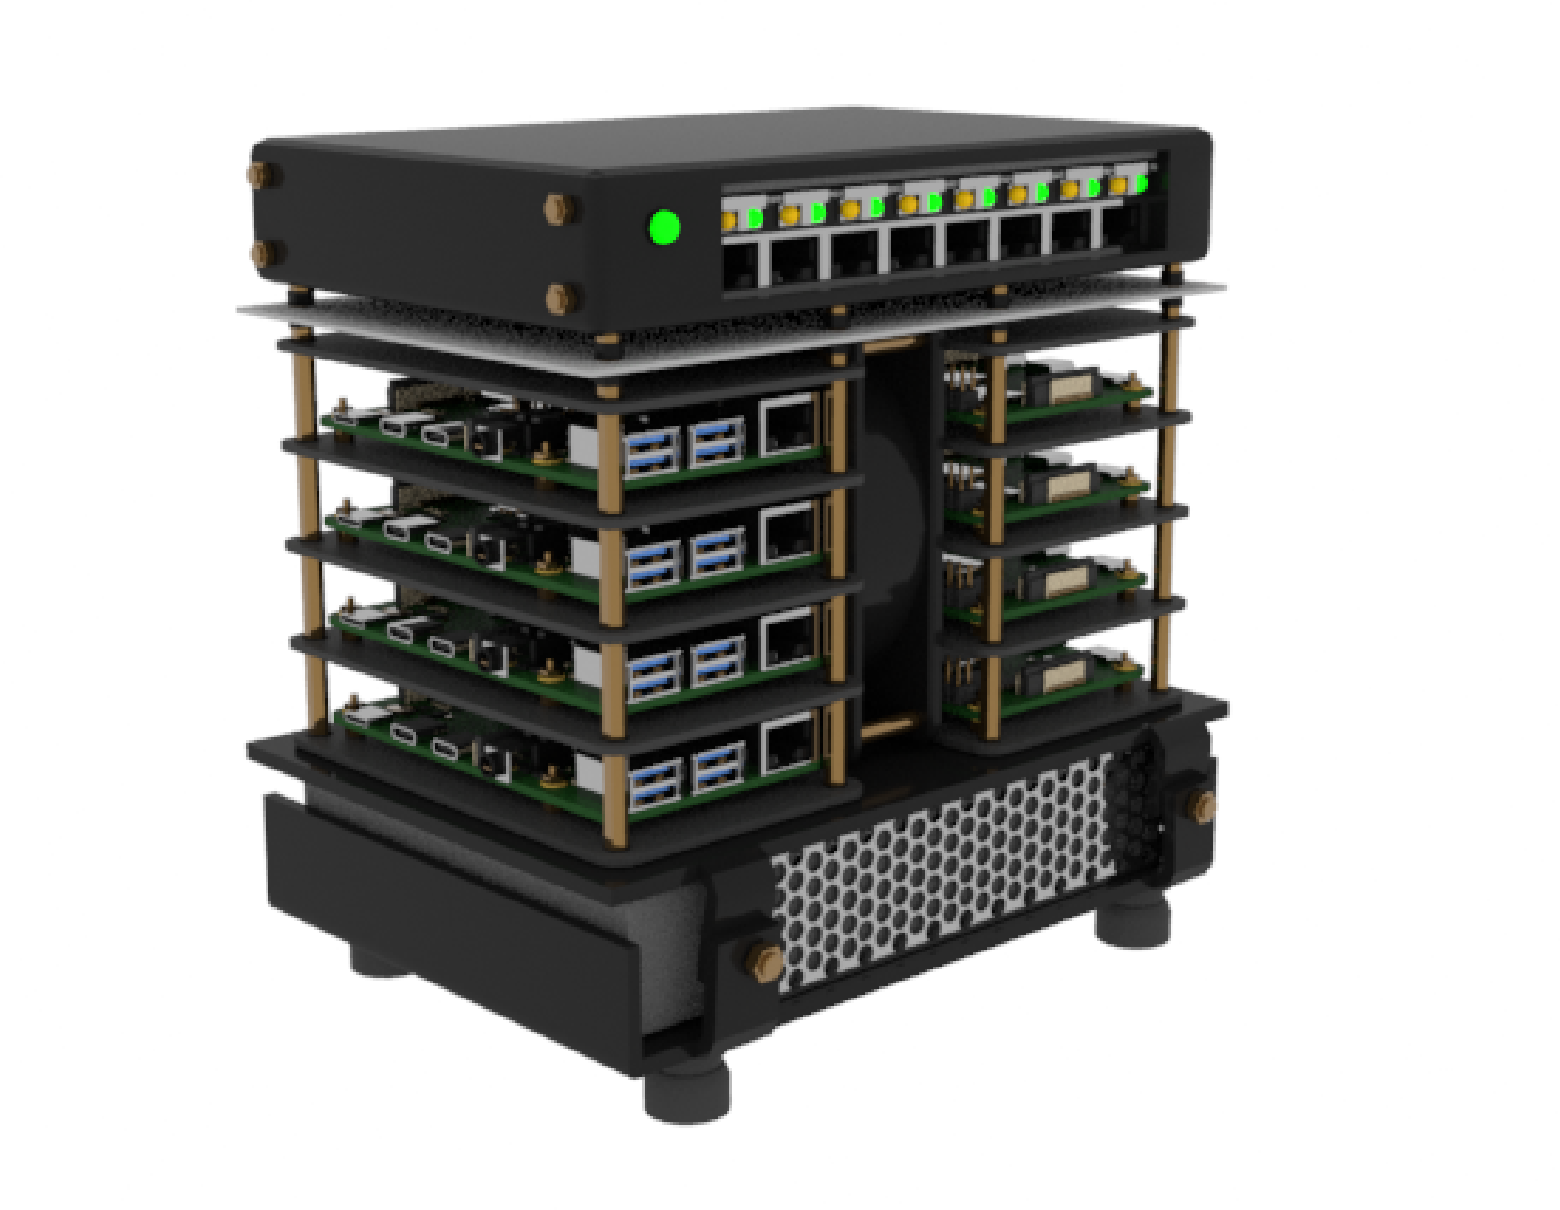
\includegraphics[width=0.8\textwidth]{img/render_cluster_1_provisional.png}
  \caption{Render frontal del cluster}
  \label{fig:render_cluster_1}
\end{figure}

El acoplamiento entre las capas se realiza mediante láminas de aluminio, en las que se atornillan las piezas de arriba y de abajo, sirviendo como adaptador.

% TODO QUIZÁS PONER QUE SE ANEXAN PLANOS CAD?

\section{Infraestructura Software}
\label{sec:infra_software}

\subsection{Requisitos funcionales}

\subsection{Requisitos no funcionales}
